\graphicspath{{./chapters/chapter05/}}
\chapter{Асимптотические свойства оценок}

Пусть $X^{(n)}=(X_1, \dots, X_n)^T$ -- вектор случайных величин на пространстве $\mathcal{X}_n=\mathcal{X}^n$ с распределением $\mathcal{P}^n=\{P_\vartheta^n \mid \vartheta \in \Theta \} $. Для любого $n$ пусть функция
\[ T_n :
\left \{
\begin{array}{ccl}
\mathcal{X}_n & \rightarrow & \Gamma \\
x^{(n)} & \mapsto & T_n(x^{(n)})  
\end{array}
\right.
\]
будет оценкой $\gamma(\vartheta)$. Минимальное условие для хорошей оценки -- это стремление $T_n$ к $\gamma(\vartheta)$ при растущем значении $n$.

\begin{defn}
	Пусть $T_n:\mathcal{X}_n \rightarrow \Gamma$ -- оценка $\gamma(\vartheta)$, принимающая значения в метрическом пространстве. Допустим, что все эксперименты определены на совместном вероятностном пространстве $P_\vartheta^n \ll Q_\vartheta$ для любого $n$.
	\begin{enumerate}
		\item $T_n$ называется \textbf{\textit{(слабо) состоятельной}} оценкой $\gamma(\vartheta)$, если 
		\[ T_n \xrightarrow{Q_\vartheta}\gamma(\vartheta) \quad \forall \vartheta \in \Theta. \]
		\item $T_n$ называется \textbf{\textit{сильно состоятельной}} оценкой $\gamma(\vartheta)$, если 
		\[ T_n \rightarrow \gamma(\vartheta) \ Q_\vartheta\text{-п.н.} \quad \forall \vartheta \in \Theta. \]
	\end{enumerate} 
\end{defn}

\begin{exmp} \label{exmp5.2}
	Вспомним метод моментов из Замечания \ref{rmrk2.41}: $X_1, \dots, X_n$ i.i.d. $\sim P_\vartheta$ вещественные случайные величины, $\vartheta \in \Theta \subset \MR^k$ и $\gamma : \Theta \rightarrow \Gamma \subset \MR^l$. Также $m_j = \ME_\vartheta[X_1^j] = \int x^j P_\vartheta(dx)$, $j = 1, \dots, k$ и 
	\[\gamma(\vartheta) = f(m_1, \dots, m_k).\]
	Далее берем
	\[ \hat{\gamma}(X) = f(\hat{m}_1, \dots, \hat{m}_k), \]
	гду $\hat{m}_j = \frac{1}{n} \sum_{i=1}^{n}X_k^j$. Если $\ME_\vartheta[|X|^k] < \infty$, то из Закона Больших чисел следует, что $\hat{m}_j \rightarrow m_j$ $Q_\vartheta$-п.н., где $Q_\vartheta = \otimes_{i=1}^\MN P_\vartheta$. Так как $f$ -- непрерывная, мы получаем:
	\[ \hat{\gamma}(X) \rightarrow \gamma(\vartheta) \quad Q_\vartheta\text{-п.н.}\]
\end{exmp}

\begin{thm}[\textbf{Теорема Крамера-Вольда}] \label{Cramer Wold}
	Пусть $(X_n)$ -- последовательность $d$-мерных случайных величин. Тогда $X_n \convdistr X$ тогда и только тогда, когда 
	\[ y^TX_n \convdistr y^TX \quad \forall y \in \MR^d. \]
\end{thm}
\begin{proof}
	Согласно Теореме Леви о непрерывности:
	\[ X_n \convdistr X\quad \Longleftrightarrow \quad \ME[\exp\{iu^tX_n\}] \rightarrow \ME[\exp\{iu^tX\}] \quad \forall u \in \MR^d. \]
	Остается только произвести замену $u=ty$ для $t \in \MR$ и $y \in \MR^d$.
\end{proof}

\begin{thm}[\textbf{Центральная предельная теорема}] \label{CLT}
	Пусть $X_1, \dots, X_n$ i.i.d. $d$-размерные случайные величины, $\ME[X_j]=\mu \in \MR^d$ и $\Cov(X_j)=\Sigma>0 \in \MR^{d \times d}$ (положительно-определенная). Тогда для случайного вектора
	\[ Z^{(n)} = \frac{1}{n}\sum_{j=1}^n \in \MR^d \]
	имеет место сходимость:
	\begin{equation} \label{CLT equation}
	\sqrt{n}(Z^{(n)}-\mu) \convdistr \mathcal{N}(0, \Sigma).
	\end{equation}
\end{thm}
\begin{proof}
	Из одномерной центральной предельной теоремы мы знаем, что
	\[ \sqrt{n}(y^TZ^{(n)}-y^T\mu) \convdistr \mathcal{N}(0, y^T\Sigma y). \]
	Применяем Теорему \ref{Cramer Wold} и получаем сходимость \eqref{CLT equation}.
\end{proof}

\begin{defn}
	Пусть $T_n:\mathcal{X}_n \rightarrow \Gamma \subset \MR^l$ -- последовательность оценок.
	\begin{enumerate}
		\item Пусть $\mu_n(\vartheta)=\ME_\vartheta[T_n]$, тогда $T_n$ называется \textbf{\textit{асимптотически несмещенной}} оценкой $\gamma(\vartheta)$, если
		\[ \mu_n(\vartheta) \rightarrow \gamma(\vartheta). \]
		\item $T_n$ назывется \textbf{\textit{асимптотически нормальной}}, если существуют последовательности $(\mu_n) \in \MR^l$ и $(\Sigma_n(\vartheta)) \in \MR^{l \times l}$, такие что $\|\Sigma_n(\vartheta) \| \rightarrow 0$ и
		\[ \Sigma_n^{-\frac{1}{2}}(\vartheta)(T_n-\mu_n(\vartheta)) \convdistr \mathcal{N}(0, \mathbb{I}_l). \]
	\end{enumerate}
\end{defn}

\begin{thm}[\textbf{Лемма Слуцкого}] \label{Slutsky}
	Пусть $(Y_n)$ и $(Z_n)$ -- последовательности $d$-мерных случайных величин, такие что 
	\[ Z_n \convdistr Z \quad \text{и} \quad Y_n \convprob y_0. \]
	Тогда:
	\begin{enumerate}
		\item $Z_n+Y_n \convdistr Z + y_0.$
		\item $Y_n^TZ_n \convdistr y_0^TZ.$
	\end{enumerate}
\end{thm}

\begin{proof}
	Теорема 11.2.11 в \cite{LehmannRomano}.
\end{proof}

\begin{exmp}
	Пусть $X_1, \dots, X_n$ i.i.d. $\sim \operatorname{Bin}(1,p)$, $p \in (0,1)$. Тогда оценка $p$ $T_n=\overline{X}_n$ является несмещенной. Из центральной предельной теоремы мы знаем, что:
	\[ \frac{\sqrt{n}(\overline{X}_n-p)}{\sqrt{p(1-p)}} \convdistr \mathcal{N}(0,1). \]
	Но так как $X_n \convprob p$, то имеет место:
	\[ \sqrt{\overline{X}_n(1-\overline{X}_n)} \convprob \sqrt{p(1-p)}. \]
	По Теореме \ref{Slutsky}:
	\[ \frac{\sqrt{n}(\overline{X}_n-p)}{\sqrt{\overline{X}_n(1-\overline{X}_n)}} \convdistr \mathcal{N}(0,1). \]
	Например, пусть $n=100$ и $\overline{X}_n=0.85$. Тогда
	\[ P_p(|\overline{X}_n-p|<\varepsilon) \approx 2 \Phi\Bigg(\varepsilon\sqrt{\frac{n}{\overline{X}_n(1-\overline{X}_n)}}\Bigg) -1 \quad \forall p \in (0, 1), \]
	где $\Phi$ -- функция распределения $\mathcal{N}(0,1)$.
	\[ P_p(|\overline{X}_n-p|<\varepsilon) \approx
	\left \{
	\begin{array}{cl}
	83.84 \%,  & \varepsilon = 0.05 \\
    99.46 \%,  & \varepsilon = 0.1  
	\end{array}
	\right.
	\]
\end{exmp}

\begin{thm}[\textbf{Дельта-метод}] \label{Delta-method}
	Пусть $(X_n)$ -- последовательность $k$-мерных случайных векторов, такая что:
	\[ \frac{X_n-\mu}{c_n} \convdistr \mathcal{N}(0, \Sigma),  \]
	где $c_n \rightarrow 0$, $\mu \in \MR^k$ и $\Sigma \geq 0 \in \MR^{k \times k}$. Пусть также $g:\MR^k \rightarrow \MR^m$ -- непрерывно дифференцируемая по $\mu$ функция с матрицей Якоби $D \in \MR^{m \times k}$. Тогда:
	\[ \frac{g(X_n)-g(\mu)}{c_n} \convdistr \mathcal{N}(0, D\Sigma D^T).  \]
\end{thm}
\begin{proof}
	По Лемме \ref{Slutsky}:
	\[	X_n-\mu = \frac{X_n-\mu}{c_n}c_n \convdistr 0.	\]
	Из сходимости по распределению к постоянной следует сходимость по вероятности:
	\[ X_n \convprob \mu. \]
	Далее
	\[ \frac{g(X_n)-g(\mu)}{c_n}=g'(\mu)\frac{X_n-\mu}{c_n}+(g'(\xi_n)-g'(\mu))\frac{X_n-\mu}{c_n}, \]
	где $\xi_n$ -- промежуточная точка:
	\[ \|\xi_n-\mu \| \leq \|X_n-\mu \|. \]
	Следовательно, $\xi_n \convprob \mu$ и $g'(\xi_n) \convprob g'(\mu)$ (поскольку $g$ -- непрерывно дифференцируемая). Вновь по Лемме \ref{Slutsky}:
	\[ g'(\mu) \frac{X_n-\mu}{c_n} \convdistr g'(\mu)\mathcal{N}(0, \Sigma). \]
\end{proof}

\begin{rmrk}
	Пусть в Примере \ref{exmp5.2} $\ME_\vartheta[X_1^{2k}] < \infty$ для любого $\vartheta \in \Theta$ и $\gamma:\MR^k \rightarrow \MR^l$ -- непрерывно дифференцируема по $\mu = (m_1, \dots, m_k)^T$ с матрицей Якоби $D$. Мы знаем из Теоремы \ref{CLT}, что
	\[ \sqrt{n}((\hat{m}_1, \dots, \hat{m}_k)^T - (m_1, \dots, m_k)^T) \convdistr \mathcal{N}(0, \Sigma),  \]
	где
	\[ \Sigma = (\Sigma)_{i,j=1}^k = (m_{i+j} - m_i m_j)_{i,j=1}^k. \]
	Тогда
	\[ \sqrt{n}(\gamma(\hat{m}_1, \dots, \hat{m}_k) - \gamma(m_1, \dots, m_k)) \convdistr \mathcal{N}(0, D \Sigma D^T).\]
\end{rmrk}

\begin{exmp}\
	\begin{enumerate}
		\item Пусть $X_1, \dots X_n$ i.i.d., $\ME_\vartheta[X_i]=\mu$ и $\Var_\vartheta(X_i)=\sigma^2$. Из ЦПТ следует:
		\[ \sqrt{n}(\overline{X}_n - \mu) \convdistr \mathcal{N}(0, \sigma^2). \]
		В качестве оценки $\mu^2$ выберем асимптотически несмещенную статистику $\overline{X}_n^2$. Используя Дельта-метод, получаем:
		\[ \sqrt{n}(\overline{X}_n^2-\mu^2) \convdistr \mathcal{N}(0, 4\mu^2\sigma^2). \]
		\item Пусть \[(X_i, Y_i)^T \sim \mathcal{N}
		\begin{pmatrix}
		\begin{pmatrix}
		\mu_1 \\ \mu_2
		\end{pmatrix},
		\begin{pmatrix}
		\sigma^2 & \rho \sigma \tau \\
		\rho \sigma \tau & \tau^2
		\end{pmatrix}
		\end{pmatrix}, \quad
		i = 1, \dots, n \] i.i.d. с параметром $\vartheta = (\mu_1, \mu_2, \sigma^2, \tau^2, \rho)^T$. Оценка
		\[ \hat{\rho}_n = \frac{SQ_{xy}}{\sqrt{SQ_{xx} SQ_{yy}}},  \]
	    где $SQ_{xy} = \frac{1}{n} \sum_{i=1}^{n}(X_i-\overline{X}_n)(Y_i - \overline{Y}_n)$, ($SQ_{xx}, SQ_{yy}$ -- аналогично), называется \textbf{\textit{коэффициентом корреляции Пирсона}}. Без ограничения общности, пусть $\mu_1 = \mu_2 = 0$, $\sigma = \tau = 1$, так как $\hat{\rho}_n$ инвариантна по отношению к аффинным преобразованиям. Докажем сначала, что $S_n = (SQ_{xx}, SQ_{yy}, SQ_{xy})^T$ удовлетворяет
	    \begin{equation} \label{5.2}
	    	 \sqrt{n}(S_n - m) \convdistr \mathcal{N}(0, V),
	    \end{equation}
	    где $m=(1, 1, \rho)^T$ и
	    \[ 
	    V = 2 
	    \begin{pmatrix}
	    1 & \rho^2 & \rho \\
	    \rho^2 & 1 & \rho \\
	    \rho & \rho & (1 + \rho^2)/2
	    \end{pmatrix}.
	    \]
	    Чтобы доказать (\ref{5.2}), используем Лемму \ref{Slutsky} и ЦПТ и покажем, что
	   \[ \sqrt{n}(\overline{X}_n, \overline{Y}_n) \convprob 0, \quad \sqrt{n}(\overline{X}_n)^2 \convprob 0, \quad \sqrt{n}(\overline{Y}_n)^2 \convprob 0.  \]
	   Далее, несложно увидеть, что
	   \[ \sqrt{n}(S_n - m) - \sqrt{n}\Big(\frac{1}{n}\sum_{i=1}^{n}Z_i - m \Big) \convprob 0, \]
	   где $Z_i = (X_i^2, Y_i^2, X_iY_i)^T$.
	   Затем, покажем, что
	   \[\Cov(Z_i) = \ME[Z_i Z_i^T]-\ME[Z_i]\ME[Z_i]^T = V. \]
	   Сходимость (\ref{5.2}) следует из Теоремы \ref{CLT}. Наконец, $g(S_n)=\hat{\rho}_n$, где $g(x_1, x_2, x_3) = \frac{x_3}{\sqrt{x_1 x_2}}$. Тогда матрица Якоби функции $g$ в точке $m$:
	   \[ D = (-\rho/2, -\rho/2, 1).\]
	   Как результат,
	   \[ \sqrt{n}(\hat{\rho}_n - \rho) \convdistr \mathcal{N}(0, DVD^T) = \mathcal{N}(0, (1-\rho^2)^2). \] 
	\end{enumerate}
\end{exmp}

\begin{defn}
	Пусть $T_n: \mathcal{X} \rightarrow \MR^l$ -- асимптотически несмещенная и асимптотически нормальная последовательность оценок. При условиях регулярности из Теоремы \ref{Cramer-Rao inequality} мы назовем $T_n$ \textbf{\textit{асимптотически эффективной}}, если
	\[ \lim\limits_{n \rightarrow \infty} \Sigma_n(\vartheta) I(f_n(\cdot, \vartheta))=\mathbb{I}_l \quad \forall \vartheta \in \Theta,  \]
	где $\mathbb{I}_l$ -- единичная матрица, а $I(f_n(\cdot, \vartheta))$ -- информация Фишера.
\end{defn}

\begin{rmrk}
	Заданное выше определение можно интерпретировать следующим образом: если $T_n$ несмещенная, то вследствие Теоремы Рао-Крамера
	\[ \Cov_\vartheta(T_n) \geq I^{-1}(f_n(\cdot, \vartheta)). \]
	Но, так как
	\[ \Sigma_n^{\frac{1}{2}} (\vartheta)(T_n - \mu_n(\vartheta)) \convdistr \mathcal{N}(0, \mathbb{I}_l), \]
	то
	\[ \Cov_\vartheta(T_n) \approx \Sigma_n(\vartheta) \approx I^{-1}(f_n(\cdot, \vartheta)) \]
	и $T_n$ асимптотически несмещенная и асимптотически эффективная. 
\end{rmrk}

\begin{exmp}
	Пусть $X_1, \dots, X_n$ i.i.d. $\sim \mathcal{N}(\mu, \sigma^2)$. Из Примера \ref{exmp2.29} следует, что для
	\[ g_n(X) = \begin{pmatrix}
	\overline{X}_n \\
	\frac{1}{n-1} \sum_{i=1}^{n} (X_i - \overline{X}_n)^2
	\end{pmatrix}  \]
	выполняется равенство
	\[ \Cov_\vartheta(g_n) = \begin{pmatrix}
	\sigma^2/n & 0 \\
	0 & 2\sigma^4 / (n - 1)
	\end{pmatrix}  
	= \Sigma_n(\vartheta). \]
	Но информация Фишера:
	\[ I^{-1}(f_n(\cdot, \vartheta)) = \begin{pmatrix}
	\sigma^2/n & 0 \\
	0 & 2\sigma^4 / n
	\end{pmatrix}   \]
	и $g_n$ не эффективная, но эффективная асимптотически.
\end{exmp}

\begin{rmrk}
	Пусть $X_1, \dots, X_n$ i.i.d. $\sim P_\vartheta$, $\vartheta \in \Theta$ с $\mu$-плотностями $f(\cdot, \vartheta)$. Мы назовем
	\[ \ell(\cdot, \vartheta) = \log f(\cdot, \vartheta)  \] 
	\textbf{\textit{логарифмической функцией правдоподобия}} и зададим
	\[ \hat{\theta}_n(X) = \arg \sup_{\vartheta \in \Theta} f(X, \vartheta) = \arg \sup_{\vartheta \in \Theta} \ell (X, \vartheta) = \arg \sup_{\vartheta \in \Theta} \frac{1}{n} \sum_{i=1}^{n} \ell (X_i, \vartheta) \]
	как оценку максимального правдоподобия для $\vartheta$ (если таковая существует).
\end{rmrk}

\begin{defn}
	Пусть $\mathbb{P}$ и $\mathbb{Q}$ -- вероятностные меры на $(\mathcal{X}, \mathcal{B})$, тогда
	\[ KL(\mathbb{P}|\mathbb{Q}) =
	\left \{
	\begin{array}{cl}
	\int_{\mathcal{X}} \log\Big(\frac{d\mathbb{P}}{d\mathbb{Q}}\Big)(x)  d\mathbb{P}(x), & \text{если } \mathbb{P} \ll \mathbb{Q}, \\
	\infty, & \text{иначе}  
	\end{array}
	\right.
	\]
	называется \textbf{\textit{расстоянием Кульбака - Лейблера}} для $\mathbb{P}$ и $\mathbb{Q}$.
\end{defn}

\begin{lmm} \label{Non-negativity of KL}
	Величина $KL(\MP|\mathbb{Q}) \geq 0$ и достигает нуля тогда и только тогда, когда $\MP = \mathbb{Q}$.
\end{lmm}
\begin{proof}
	\[
	\begin{aligned}
	\int_{\mathcal{X}} \log \Big(\frac{d\MP}{d\mathbb{Q}}\Big)(x) \MP(dx) & = \int_{\mathcal{X}} - \log\Big(\frac{d\mathbb{Q}}{d\MP}\Big)(x) \MP(dx) \\
	\text{неравенство Йенсена} \rightarrow & \geq  -\log \int_{\mathcal{X}} \Big(\frac{d\mathbb{Q}}{d\MP}\Big)(x) \MP(dx) \\
	& = -\log \int_{\mathcal{X}} \mathbb{Q}(dx) = 0.
	\end{aligned}
	 \]
	 Неравенство вырождается в равенство, если $\frac{d\mathbb{Q}(x)}{d\MP(x)}=1$ п.н.
\end{proof}

\begin{thm} \label{Consistency of ML estimator}
	Пусть $X_1, \dots, X_n$ i.i.d. $\sim P_\vartheta$, $\vartheta \in \Theta$, $\ell(\cdot, \vartheta)$ -- функция правдоподобия. Также:
	\begin{enumerate}
		\item $\Theta \subset \MR^k$ -- компактное пространство.
		\item $\eta \mapsto L(\eta, \vartheta) = \ME[\ell(X_i, \eta)]$ непрерывная и $\eta \mapsto L_n(\eta) = \frac{1}{n}\sum_{i=1}^n\ell(X_i, \eta)$ $\otimes_{i=1}^nP_\vartheta$-п.н. непрерывная функции.
		\item Пусть $Q_\vartheta=\otimes_{i=1}^\MN P_\vartheta$ и
		\[ \sup_{\eta \in \Theta} | L_n(\eta)-L(\eta, \vartheta)|\xrightarrow{Q_\vartheta}0. \]
	\end{enumerate}
	Тогда оценка максимального правдоподобия $\hat{\theta}_n$ состоятельная.
\end{thm}
\begin{proof}
	Для любого $\eta \in \Theta$:
	\[ L_n(\eta) \rightarrow L(\eta, \vartheta) = \int \ell(x, \eta) f(x,\vartheta) \mu(dx) = \int \ell(x,\vartheta)f(x,\vartheta)\mu(dx) - KL(\vartheta | \eta)  \]
	$\mu$-п.н. Используя Лемму \ref{Non-negativity of KL}, заключаем что $\eta \mapsto L(\eta, \vartheta)$ достигает максимума при $\eta = \vartheta$. Функция
	\[ \arg \max : 
	\left \{
	\begin{array}{ccl}
	 C(\Theta, \MR) & \rightarrow & \Theta \\
	 f & \mapsto & m_f = \arg \max_{\eta \in \Theta} f(\eta)
	\end{array}
	\right.
	 \]
	 непрерывна для тех $f$, для которых $m_f$ единственная. Тогда утверждение будет доказано, исходя из того, что
	 \[ \vartheta = \arg \max L(\eta, \vartheta)\quad \text{и} \quad \hat{\theta}_n=\arg \max L_n(\eta)  \]
	 и из условия (iii).
\end{proof}

\begin{rmrk} \
	\begin{enumerate}
		\item Так как $\eta \rightarrow L_n(\eta)$ (п.н.) непрерывна и $\Theta$ -- компакт, оценка максимального правдоподобия существует (п.н.) и измерима (Лемма 6.7 в \cite{WittingMuller})
		\item Наиболее сложным условием для проверки является условие (iii). Обычно используется следующий вывод: \\
		Предположим, что $T \subset \MR$ компакт и случайные величины $X_n(\gamma)$ и $X(\gamma)$ такие, что
		\begin{center}\centering
			\begin{minipage}{0.65\linewidth}
				\[ X_n(\gamma) \convprob X(\gamma) \]
				и
				\[ \gamma \mapsto X(\gamma) \quad \text{и} \quad \gamma \mapsto X_n(\gamma) \]
				(п.н.) непрерывные. Тогда
				\[ \sup_{\gamma \in \Gamma} \| X_n(\gamma) - X(\gamma) \| \convprob 0 \]
			\end{minipage}
			\begin{minipage}{0.32\textwidth}
				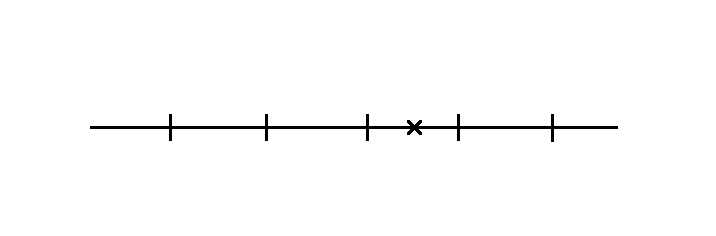
\includegraphics[width=\linewidth, height=1.5cm, right]{interpolation}
				\captionsetup{labelformat=empty}
				\put(-68, 27){$\gamma$}
				\put(-75, 16){$\underbrace{}$} 
				\put(-68, 0){$\delta$} \
				Идея заключается в интерполяции внутри интервалов $\delta$.
			\end{minipage}
		\end{center}
		тогда и только тогда, когда
		\[ \forall \varepsilon > 0 \quad \lim_{\delta \rightarrow 0} \limsup_{n \rightarrow \infty} \MP \bigg(\sup_{| \gamma_1 - \gamma_2 | < \delta} \| X_n(\gamma_1) - X_n(\gamma_2) \| \geq \varepsilon \bigg) = 0. \]
    \end{enumerate}
\end{rmrk}

\begin{thm}[\textbf{Асимптотическая эффективность оценок МП}] \label{Asymptotic efficiency ML estimators}
	Пусть $X_1, \dots, X_n$ i.i.d. $\sim P_\vartheta$, $\vartheta \in \Theta$, $\ell(\cdot, \vartheta)$ -- функция правдоподобия. Также:
	\begin{enumerate}
		\item $\Theta \subset \MR^k$ -- компактное пространство и $\vartheta \subset \operatorname{int}(\Theta)$.
		\item $\eta \mapsto \ell(x, \eta) $ непрерывна на $\Theta$ и дважды непрерывно дифференцируема по $\vartheta$ для почти всех $x \in \mathcal{X}$.
		\item Существуют функции $H_0, H_2 \in L^1(P_\vartheta)$ и $H_1 \in L^2(P_\vartheta)$, такие что:
		\[ \sup_{\eta \in \Theta} |\ell(x, \eta)| \leq H_0(x), \quad \sup_{\eta \in \Theta} \|\dot{\ell}(x, \eta)\| \leq H_1(x), \quad \sup_{\eta \in \Theta} \|\ddot{\ell}(x, \eta)\| \leq H_2(x) \quad \forall x \in \mathcal{X}. \]
		\item Информация Фишера
		\[ I(f(\cdot, \vartheta))=\ME_\vartheta[\dot{\ell}(X,\vartheta)\dot{\ell}(X,\vartheta)^T] \]
		положительно определенная (обратима).
	\end{enumerate}
	Тогда имеет место сходимость:
	\[ \sqrt{n}(\hat{\theta}_n-\vartheta) \convdistr \mathcal{N}(0, I(f(\cdot, \vartheta))^{-1}). \]
\end{thm}
\begin{proof} \\
	\textit{Шаг 1:} покажем состоятельность оценки $\hat{\theta}_n$ (проверим, что условия из Теоремы \ref{Consistency of ML estimator} соблюдаются)
	\begin{enumerate}
		\item Соблюдается по предположению.
		\item $\eta \mapsto L_n(\eta)$ п.н. непрерывная по условию (ii). Также, используя (ii), (iii) и мажорируемую сходимость, получаем
		\[ |L(\eta_1, \vartheta) - L(\eta_2, \vartheta)| \leq \int_{\mathcal{X}} |\ell(x, \eta_1) - \ell(x,\eta_2)| f(x,\vartheta) \mu(dx) \rightarrow 0,  \]
		при $\eta_1 \rightarrow \eta_2$.
		\item В силу Сильного Закона Больших Чисел:
		\[
		\begin{aligned}
		\limsup_{n \rightarrow \infty} \sup_{\| \eta_1 - \eta_2 \| < \delta} | L_n(\eta_1) - L_n(\eta_2)| & \leq \limsup_{n \rightarrow \infty} \frac{1}{n} \sum_{i=1}^{n} \sup_{\| \eta_1 - \eta_2 \| < \delta} |\ell(X_i, \eta_1) - \ell(X_i, \eta_2) |\\
		& = \ME_\vartheta[\sup_{\| \eta_1 - \eta_2 \| < \delta}|\ell(X,\eta_1) - \ell(X, \eta_2)|] \quad Q_\vartheta = \otimes_{i=1}^\MN P_\vartheta\text{-п.н.}
		\end{aligned}
		\]
		Так как $\Theta$ компакт, то $\eta \mapsto \ell(X, \eta)$ (п.н.) равномерно непрерывная. Как следствие, последнее выражение сходится к нулю при $\delta \rightarrow 0$ (используя снова мажорируемую сходимость).
	\end{enumerate}	

	\textit{Шаг 2:} пусть $A_n$ -- $k$-мерный прямоугольник с вершинами $\hat{\theta}_n$ и $\vartheta$. Поскольку $\hat{\theta}_n \xrightarrow{Q_\vartheta} \vartheta$ и $\vartheta \in \operatorname{int}(\Theta)$, то
	\[ Q_\vartheta(A_n \subset \operatorname{int}(\Theta)) \rightarrow 1. \]
	Также
	\[ \dot{L}_n(\hat{\theta}_n) = \frac{1}{n} \sum_{i=1}^{n} \dot{\ell}(X_i, \hat{\theta}_n) = 0 \]
	по определению $\hat{\theta}_n$.
	По Теореме о среднем:
	\[ -\dot{L}_n(\vartheta) = \dot{L}_n(\hat{\theta}_n) - \dot{L}_n(\vartheta) = \ddot{L}_n(\widetilde{\theta}_n)(\hat{\theta}_n - \vartheta) \]
	для некоторого $\widetilde{\theta}_n \in A_n$.
	Как и в Замечании \ref{rmrk2.25}:
	\[
	\begin{aligned}
	 \ME[\dot{\ell}(X_i, \vartheta)] & = \int_{\mathcal{X}} \dot{\ell}(x, \vartheta) f(x, \vartheta) \mu(dx) \\
	 \ell = \log f \rightarrow & = \int_{\mathcal{X}} \dot{f}(x, \vartheta) \mu(dx) = 0.
	\end{aligned}
	 \]
	 По определению
	 \[ \Cov(\dot{\ell}(X_i, \vartheta)) = I(f(\cdot, \vartheta)). \]
	 Тогда по Центральной Предельной Теореме:
	 \[ \sqrt{n} \dot{L}_n(\vartheta) \convdistr \mathcal{N}(0, I(f(\cdot, \vartheta))). \]
	 
	\textit{Шаг 3:} предположим, что
	\begin{equation} \label{eq5.3}
		\ddot{L}_n(\widetilde{\theta}_n) \xrightarrow{Q_\vartheta} -I(f(\cdot, \vartheta)).
	\end{equation}
	Если \eqref{eq5.3} соблюдается, мы можем заключить, что
	\[ \lim\limits_{n \rightarrow \infty} Q_\vartheta(\ddot{L}_n(\widetilde{\theta}_n) \text{ обратима}) = 1. \]
	Тогда, используя лемму Слуцкого, получаем
	\[
	\begin{aligned}
	\sqrt{n}(\hat{\theta}_n - \vartheta) & = -\ddot{L}_n(\widetilde{\theta}_n)^{-1} \dot{L}_n(\vartheta) 1_{ \{ A_n \subset \operatorname{int}(\Theta)
	 \} \cap \{ \ddot{L}_n(\widetilde{\theta}_n) \text{ обратима} \}} + B_n \\
	& \rightarrow I(f(\cdot, \vartheta))^{-1} \mathcal{N}(0, I(f(\cdot, \vartheta))) = \mathcal{N}(0, I(f(\cdot, \vartheta))^{-1}),
	\end{aligned}
	\]
	так как $B_n \xrightarrow{Q_\vartheta} 0$.
	
	\textit{Шаг 4:} докажем \eqref{eq5.3}. Используем равенство:
	\[ \ddot{\ell}(x, \vartheta) = \frac{\ddot{f}(x, \vartheta)}{f(x,\vartheta)} - \dot{\ell}(x, \vartheta)\dot{\ell}(x, \vartheta)^T. \]
	Тогда имеет место:
	\[\ME_\vartheta[\ddot{\ell}(X, \vartheta)] + I(f(\cdot, \vartheta)) = \ME_\vartheta\Big[ \frac{\ddot{f}(X, \vartheta)}{f(X,\vartheta)} \Big] = 0, \]
	как в Замечании \ref{rmrk2.25}. Из Закона Больших Чисел следует:
	\[ \ddot{L}_n(\vartheta) \xrightarrow{Q_\vartheta} - I(f(\cdot, \vartheta)). \]
	Наконец, используем равенство
	\[ \lim\limits_{\delta \rightarrow 0} \lim\limits_{n \rightarrow \infty} Q_\vartheta(\| \widetilde{\theta}_n - \vartheta \| < \delta) = 1 \]
	и непрерывность $\ddot{\ell}$ по $\vartheta$, чтобы завершить доказательство \eqref{eq5.3}.
\end{proof}

\begin{rmrk}
	Теорема \ref{Consistency of ML estimator} и Теорема \ref{Asymptotic efficiency ML estimators} -- это специальные случаи \textbf{\textit{оценок минимального контраста}}, которые минимизируют функцию
	\[ \eta \mapsto \frac{1}{n} \sum_{i=1}^{n}k(X_i, \eta). \]
	Можно получить похожие результаты при схожих предположениях, но асимптотическая эффективность достигается только при $k = -\ell$.
\end{rmrk}

\begin{exmp}
	Пусть $X_1, \dots, X_n$ i.i.d. $\sim Exp(\lambda)$. Найдем оценку максимального правдоподобия. Для этого
	\[f_n(X, \lambda) = \lambda^n \exp\bigg(-\lambda \sum_{i=1}^{n} X_i\bigg) 1_{[0, \infty)} (\min_{i=1}^n X_i) \]
	или
	\[\ell_n(X, \lambda) = n \log(\lambda) - \lambda \sum_{i=1}^{n} X_i + \log 1_{[0, \infty)} (\min_{i=1}^n X_i) \]
	должны быть максимизированы. Приравнивая любую из производных к нулю, получаем условие:
	\[\frac{n}{\lambda} = \sum_{i=1}^{n} X_i,  \]
	то есть оценка:
	\[\hat{\lambda}_n = \frac{1}{\overline{X}_n}. \]
	Рассчитаем информацию Фишера:
	\[ 
	\begin{aligned}
	\ell_1 (X, \lambda)&  = \log(\lambda) - \lambda X + \log(1_{[0, \infty)} X) \\
	&\Rightarrow \dot{\ell}_1(X, \lambda) = -\Big(X - \frac{1}{\lambda}\Big) \\
	&\Rightarrow I(f(\cdot, \lambda)) = \ME_\lambda\Big[\Big(X - \frac{1}{\lambda}\Big)^2\Big]. 
	\end{aligned}
	\]
	По Теореме \ref{Asymptotic efficiency ML estimators}
	\[ \sqrt{n}(\hat{\lambda}_n - \lambda) \convdistr \mathcal{N}(0, \lambda^2),  \]
	но с другой стороны:
	\[ \sqrt{n}\Big(\overline{X}_n - \frac{1}{\lambda}\Big) \convdistr \mathcal{N}\Big(0, \frac{1}{\lambda^2}\Big).  \]
	Используя Дельта-метод для $g(x) = x^{-1}$, получаем
	\[ \sqrt{n}(\overline{X}_n^{-1} - \lambda) \convdistr \mathcal{N}(0, \lambda^2). \]
	Также заметим, что
	\[ \Var_\lambda(\hat{\lambda}_n) = n^{-1} \lambda^2 = (n I(f(\cdot, \lambda)))^{-1} \]
	является следствием из Предположения \ref{prps2.31} для экспоненциального семейства.
\end{exmp}

\raggedbottom
\pagebreak
\section*{Упражнения}
\begin{exc}
	Докажите следующий вариант леммы Слуцкого: пусть $(X_n)$ и $(Y_n)$ -- последовательности вещественнозначных случайных величин, такие что
	\[X_n \convdistr X \quad \text{и} \quad Y_n \convprob c,  \]
	где $X$ -- вещественнозначная случайная величина и $c \in \MR$. Тогда имеет место:
	\[ X_n + Y_n \convdistr X + c. \]
	\textit{Подсказка}: последовательность $(Z_n)$ сходится к $Z$ тогда и только тогда, когда $\ME[f(Z_n)] \rightarrow \ME[f(Z)]$ для любых равномерно непрерывных и ограниченных функций $f:\MR \rightarrow \MR$.
\end{exc}

\begin{exc}
	Пусть $(X_n)$ -- последовательность i.i.d. случайных величин с плотностью
	\[ f(x, \vartheta) = \vartheta x^{\vartheta - 1} 1_{[0, 1]}(x). \]
	\begin{enumerate}
		\item Найдите оценку максимального правдоподобия $\hat{\vartheta}$.
		\item Рассчитайте асимптотическое распределение $\hat{\vartheta}$. \\
		\textit{Подсказка}: для $\vartheta > 0$:
		\[ \int_{0}^{1} \log(x) x^{\vartheta - 1} dx = -\frac{1}{\vartheta}, \quad \int_{0}^{1} (\log(x))^2x^{\vartheta - 1}dx = \frac{2}{\vartheta^3}.  \]
	\end{enumerate}
\end{exc}

\begin{exc}
	\textbf{\textit{Коэффициент вариации}} вероятностного распределения $P$ определяется как
	\[ c_v(X) := \frac{\sqrt{\Var(X)}}{\ME[X]},\ X \sim P, \]
	если соответствующие моменты существуют и $\ME[X] \neq 0$. Пусть $(X_n)$ -- последовательность i.i.d. нормально распределенных случайных величин: $X_i \sim \mathcal{N}(\mu, \sigma^2)$, где $\mu \in \MR / \{0\}$ и $\sigma^2 > 0$.
	\begin{enumerate}
		\item Найдите оценку $\hat{c}_n(X)$ для $c_v(X)$, полученную методом моментов.
		\item Выведите Центральную Предельную Теорему для оценки $\hat{c}_n(X)$.
	\end{enumerate}
\end{exc}

\begin{exc}
	Пусть $(X_n)$ -- последовательность i.i.d. равномерно распределенных случайных величин: $X_i \sim \mathcal{U}[0. \vartheta]$. Покажите, что $\big(\prod_{i=1}^{n} X_i \big)^{\frac{1}{n}}$ -- состоятельная оценка для $\frac{\vartheta}{e}$.\\
	\subitem \textit{Подсказка}: один из способов доказать сходимость по распределению, это показать, что
	\[ \sqrt{n} \bigg(\Big(\prod_{i=1}^{n} X_i \Big)^{\frac{1}{n}} - \frac{\vartheta}{e} \bigg) \convdistr \mathcal{N}\bigg(0, \Big(\frac{\vartheta}{e} \Big)^2\bigg). \]
\end{exc}

\begin{exc}
	Пусть $(X_n)$ -- последовательность i.i.d. $\mathcal{N}(\mu, 1)$ распределенных величин. Пусть также $a > 0$ и
	\[ \hat{\mu}_a =
	\left \{
	\begin{array}{cl}
	\overline{X}_n, & |\overline{X}_n| \geq n^{-\frac{1}{4}}, \\
	a\overline{X}_n, & \text{иначе}. 
	\end{array}
	\right.
	\]
	\begin{enumerate}
		\item Покажите, что
		\[ \sqrt{n}(\hat{\mu}_a - \mu) \convdistr \mathcal{N}(0, v(\mu)), \]
		где $v(\mu) = 1$, если $\mu \neq 0$, и $v(\mu) = a^2$, иначе.
		\item Для каких $a$ $\mu_a$ является эффективной?
		\item Покажите, что существуют случаи, для которых имеет место:
		\[ v(\mu) \leq I_1^{-1}(\mu). \]
	\end{enumerate}
\end{exc}